\section{Casi d'uso}

\subsection{Obiettivi}
La sezione 3 Casi d'uso ha come obiettivo l'identificazione e la descrizione di tutti i casi d'uso, ovvero interazioni tra sistema ed attori, individuati dagli analisti nel tempo tramite lo studio del capitolato d'appalto, del dominio, e tramite incontri con il committente.

\subsection{Attori}
Dato che il requisito obbligatorio richiede la costruzione di una pagina di login(probabilmente username e password saranno preimpostati) che presenti un sistema in grado di distinguere un utente umano da un robot, il prodotto presenterà una sola tipologia di utente:\\
\begin{center}
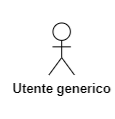
\includegraphics[scale = 1]{img/utente_generico.png}\\
\end{center}
L'utente generico, che potrà essere una persona fisica o anche un bot, potrà accedere a tutte le funzionalità del prodotto. \\
TODO aggiungere eventualmente come utenti il db di unsplash e servizi vari in futuro

\begin{center}
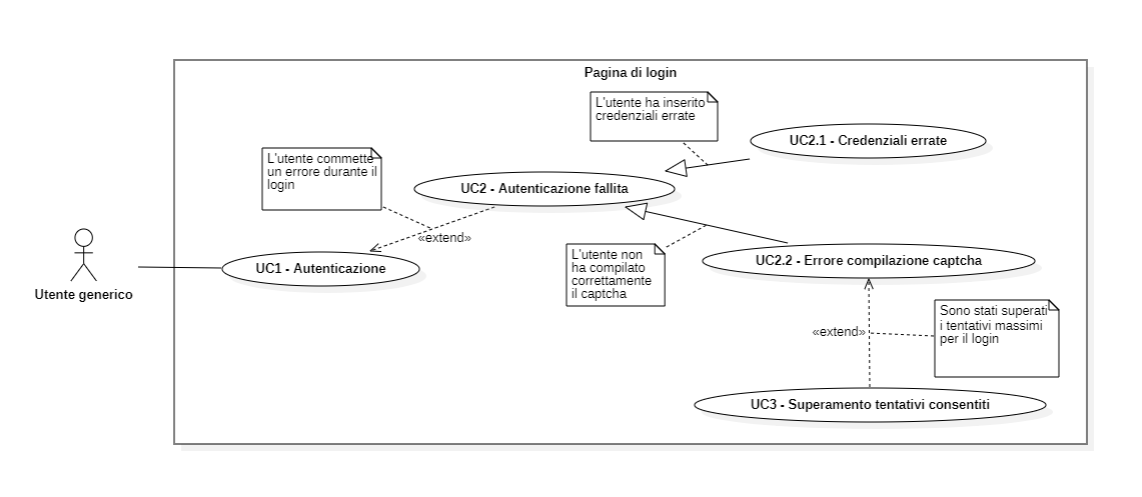
\includegraphics[scale = 0.65]{img/MainUML.png}\\
\end{center}

\subsection{UC1 - Autenticazione}
\textbf{Attore primario}: Utente generico\\
\textbf{Precondizioni}: Il sistema non riconosce l'utente\\
\textbf{Postcondizioni}: L'utente è autenticato nel sistema\\

\textbf{Scenario principale}: L'utente:
\begin{enumerate}
\item Inserisce il proprio username [UC1.1]
\item Inserisce la propria password [UC1.2]
\item Compila correttamente il captcha visualizzato [UC1.3]
\end{enumerate}

\textbf{Scenari alternativi}:
\begin{enumerate}
    \item L’utente compila in modo errato il modulo di login e gli viene mostrato un errore. [UC2]
\end{enumerate}

\begin{center}
	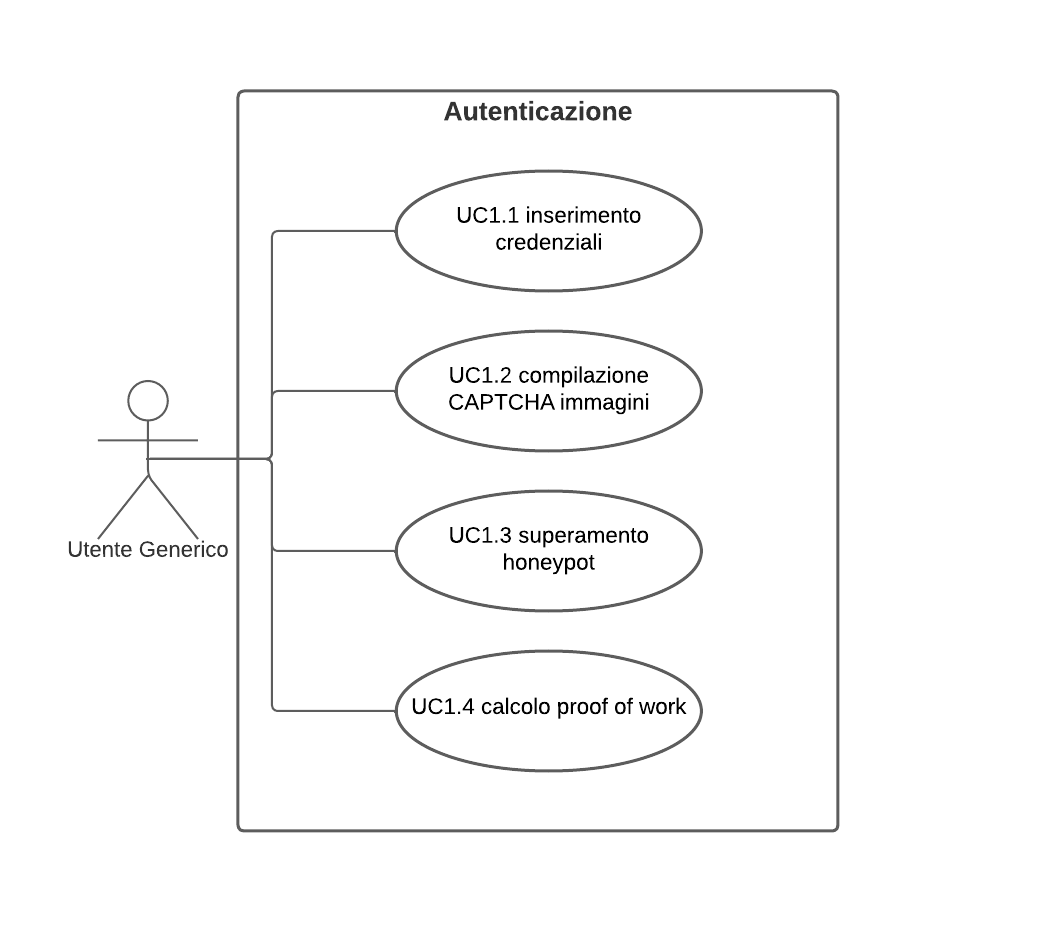
\includegraphics[scale = 1]{img/Autenticazione.png}\\
\end{center}

\subsubsection{UC1.1 - Inserimento username}
\textbf{Attore primario}: Utente generico\\
\textbf{Precondizioni}: Il sistema non riconosce l'utente e non conosce l'username\\
\textbf{Postcondizioni}: Il sistema ha ricevuto l'username dell'utente\\

\textbf{Scenario principale}:
\begin{enumerate}
   \item L'utente inserisce l'username nell'apposito spazio. L'username deve essere quello preimpostato.
\end{enumerate}

\subsubsection{UC1.2 - Inserimento password}
\textbf{Attore primario}: Utente generico\\
\textbf{Precondizioni}: Il sistema non riconosce l'utente e non conosce la password\\
\textbf{Postcondizioni}: Il sistema ha ricevuto la password dell'utente\\

\textbf{Scenario principale}:
\begin{enumerate}
   \item L'utente inserisce la password nell'apposito spazio. L'username deve essere quello preimpostato.
\end{enumerate}

\subsubsection{UC1.3 - Compilazione captcha}
\textbf{Attore primario}: Utente generico\\
\textbf{Precondizioni}: L'utente visualizza il captcha proposto dal sistema\\
\textbf{Postcondizioni}: L'utente ha risolto il captcha (non necessariamente in modo corretto)\\

\textbf{Scenario principale}:
\begin{enumerate}
   \item L'utente risolve il captcha proposto, non necessariamente in maniera corretta
\end{enumerate}
\textbf{Generalizzazioni}:
\begin{itemize}
   \item captcha tipo 1 [UC1.3.1]
   \item captcha tipo 2 [UC1.3.2]
   \item ...
\end{itemize}

\paragraph{UC1.3.1 - Compilazione captcha tipo 1 }~\smallskip
\textbf{chiedere quanto si può andare in dettaglio}\\
\textbf{Attore primario}: Utente generico\\
\textbf{Precondizioni}: L'utente visualizza il captcha tipo 1\\
\textbf{Postcondizioni}: L'utente ha completato il captcha di tipo 1\\
\textbf{Scenario principale}:

All'utente viene presentato il captcha tipo 1, con 9 immagini da classificare\\
L'utente classifica le 9 immagini nelle giuste categorie


\paragraph{UC1.3.2 - Compilazione captcha tipo 2}~\smallskip
\textbf{Attore primario}: Utente generico\\
\textbf{Precondizioni}: L'utente visualizza il captcha tipo 2\\
\textbf{Postcondizioni}: L'utente ha completato il captcha di tipo 2\\
\textbf{Scenario principale}:

All'utente viene presentato il captcha tipo 2
[elenco delle azioni che servono per superare il captcha]

\subsection{UC2 - Autenticazione fallita}
\textbf{Attore primario}: Utente generico\\
\textbf{Precondizioni}: L’utente non ha compilato correttamente il modulo di login.\\
\textbf{Postcondizioni}:L’utente visualizza un messaggio di errore e l’operazione di autenticazione fallisce.\\

\textbf{Scenario principale}:
\begin{enumerate}
   \item L’utente commette un errore nella compilazione del modulo di login.
\end{enumerate}

\textbf{Generalizzazioni}: L'utente ha commesso uno dei seguenti errori:
\begin{enumerate}
	\item Ha inserito delle credenziali errate [UC2.1]
	\item Ha sbagliato a compilare il captcha [UC2.2]
\end{enumerate}

\begin{center}
	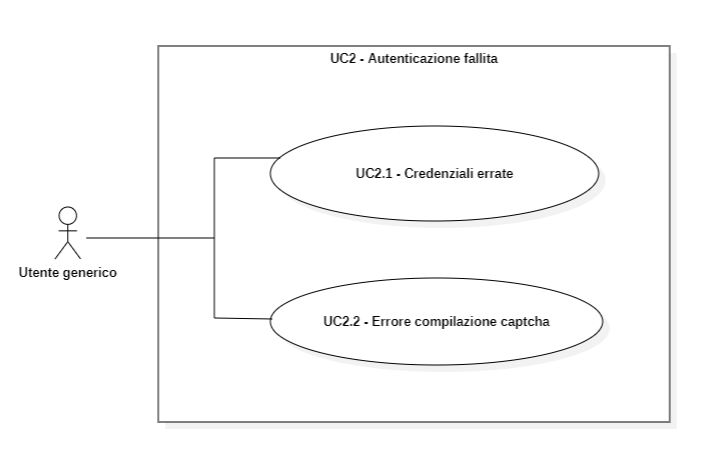
\includegraphics[scale = 0.9]{img/Autenticazione_fallita.png}\\
\end{center}

\subsubsection{UC2.1 - Credenziali errate}
\textbf{Attore primario:} Utente generico\\
\textbf{Precondizioni}: L’utente non ha inserito le credenziali corrette\\
\textbf{Postcondizioni}:  L’utente visualizza un messaggio di errore e l’operazione di autenticazione fallisce. L’utente potrà riprovare  ad autenticarsi.\\

\textbf{Scenario principale}:
\begin{enumerate}
	\item L’utente visualizza un messaggio di errore
	\item L’operazione di autenticazione fallisce
	\item Viene generato un altro captcha e l’utente potrà riprovare ad autenticarsi
\end{enumerate}

\subsubsection{UC2.2 - Errore compilazione captcha}
\textbf{Attore primario:} Utente generico\\
\textbf{Precondizioni}: L’utente non ha compilato correttamente il captcha\\
\textbf{Postcondizioni}:  L’utente visualizza un messaggio di errore e l’operazione di autenticazione fallisce. L’utente potrà riprovare  ad autenticarsi.\\

\textbf{Scenario principale}:
\begin{enumerate}
	\item Viene visualizzato un errore esplicativo
	\item Il numero di tentativi compiuti dall’utente negli ultimi 20 minuti aumenta di 1
	\item L’utente non viene autenticato nel sistema e potrà  riprovare ad autenticarsi
\end{enumerate}

\textbf{Scenario alternativo}:
\begin{enumerate}
	\item L’utente ha superato il numero di tentativi consentito per la compilazione del captcha negli ultimi 20 minuti. [UC3]
\end{enumerate}

\begin{center}
	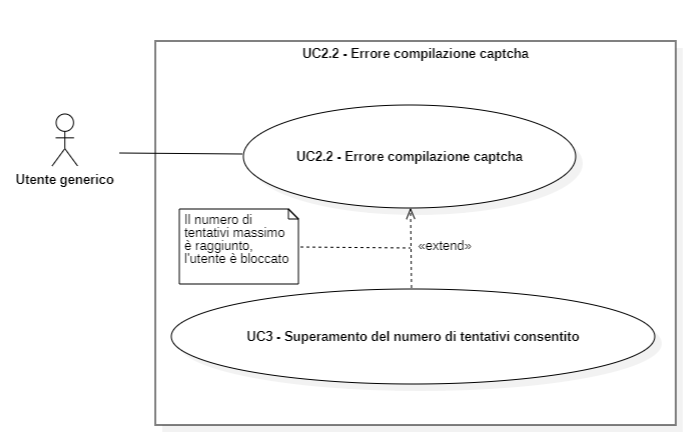
\includegraphics[scale = 0.9]{img/Errore_captcha.png}\\
\end{center}

\subsection{UC3 - Superamento del numero di tentativi consentito}
\textbf{Attore primario}: Utente generico\\
\textbf{Precondizioni}: L'utente ha superato il numero massimo di tentativi di autenticazione consentiti e non ha compilato l'ultimo captcha correttamente\\
\textbf{Postcondizioni}:L'operazione di autenticazione fallisce e l'utente viene bloccato\\

\textbf{Scenario principale}:
\begin{enumerate}
   \item L'utente visualizza un messaggio di errore che comunica lo stato di blocco
   \item L'utente conferma di aver visualizzato il messaggio di errore
   \item L'operazione di autenticazione fallisce
   \item L'utente viene bloccato da futuri tentativi di login per un tempo prestabilito
\end{enumerate}

\subsection{UC4 - Generazione di un altro captcha (da chiedere su una possibile generalizzazione)}
\textbf{Attore primario}: Utente generico\\
\textbf{Precondizioni}: L'utente ha visualizzato il captcha proposto\\
\textbf{Postcondizioni}: All'utente viene proposto un nuovo captcha\\

\textbf{Scenario principale}:
\begin{enumerate}
   \item L'utente richiede la generazione di un nuovo captcha
   \item Il sistema propone all'utente un altro captcha
\end{enumerate}

\begin{center}
	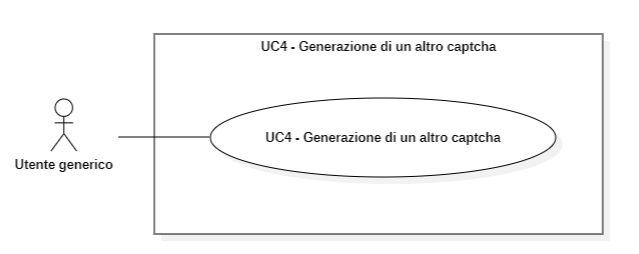
\includegraphics[scale = 0.9]{img/Generazione_captcha.png}\\
\end{center}